\section{Continuous Integration}

Nel modello a cascata, l'integrazione rappresenta una fase a sé stante. Nei primi anni dello sviluppo software si volevano seguire i modelli di integrazione:
\begin{itemize}
    \item Bottom Up: partendo dalle foglie viene ricomposto il sistema generale.
    \item Top Down: partendo dallo schema generico vengono implementate man mano le funzionalità.
\end{itemize}
In realtà, sopratutto con l’object orientation, vbiene fatto tutto un po’ alla rinfusa, senza un chiaro modello di sviluppo.
\begin{figure}[H]
	\centering
	 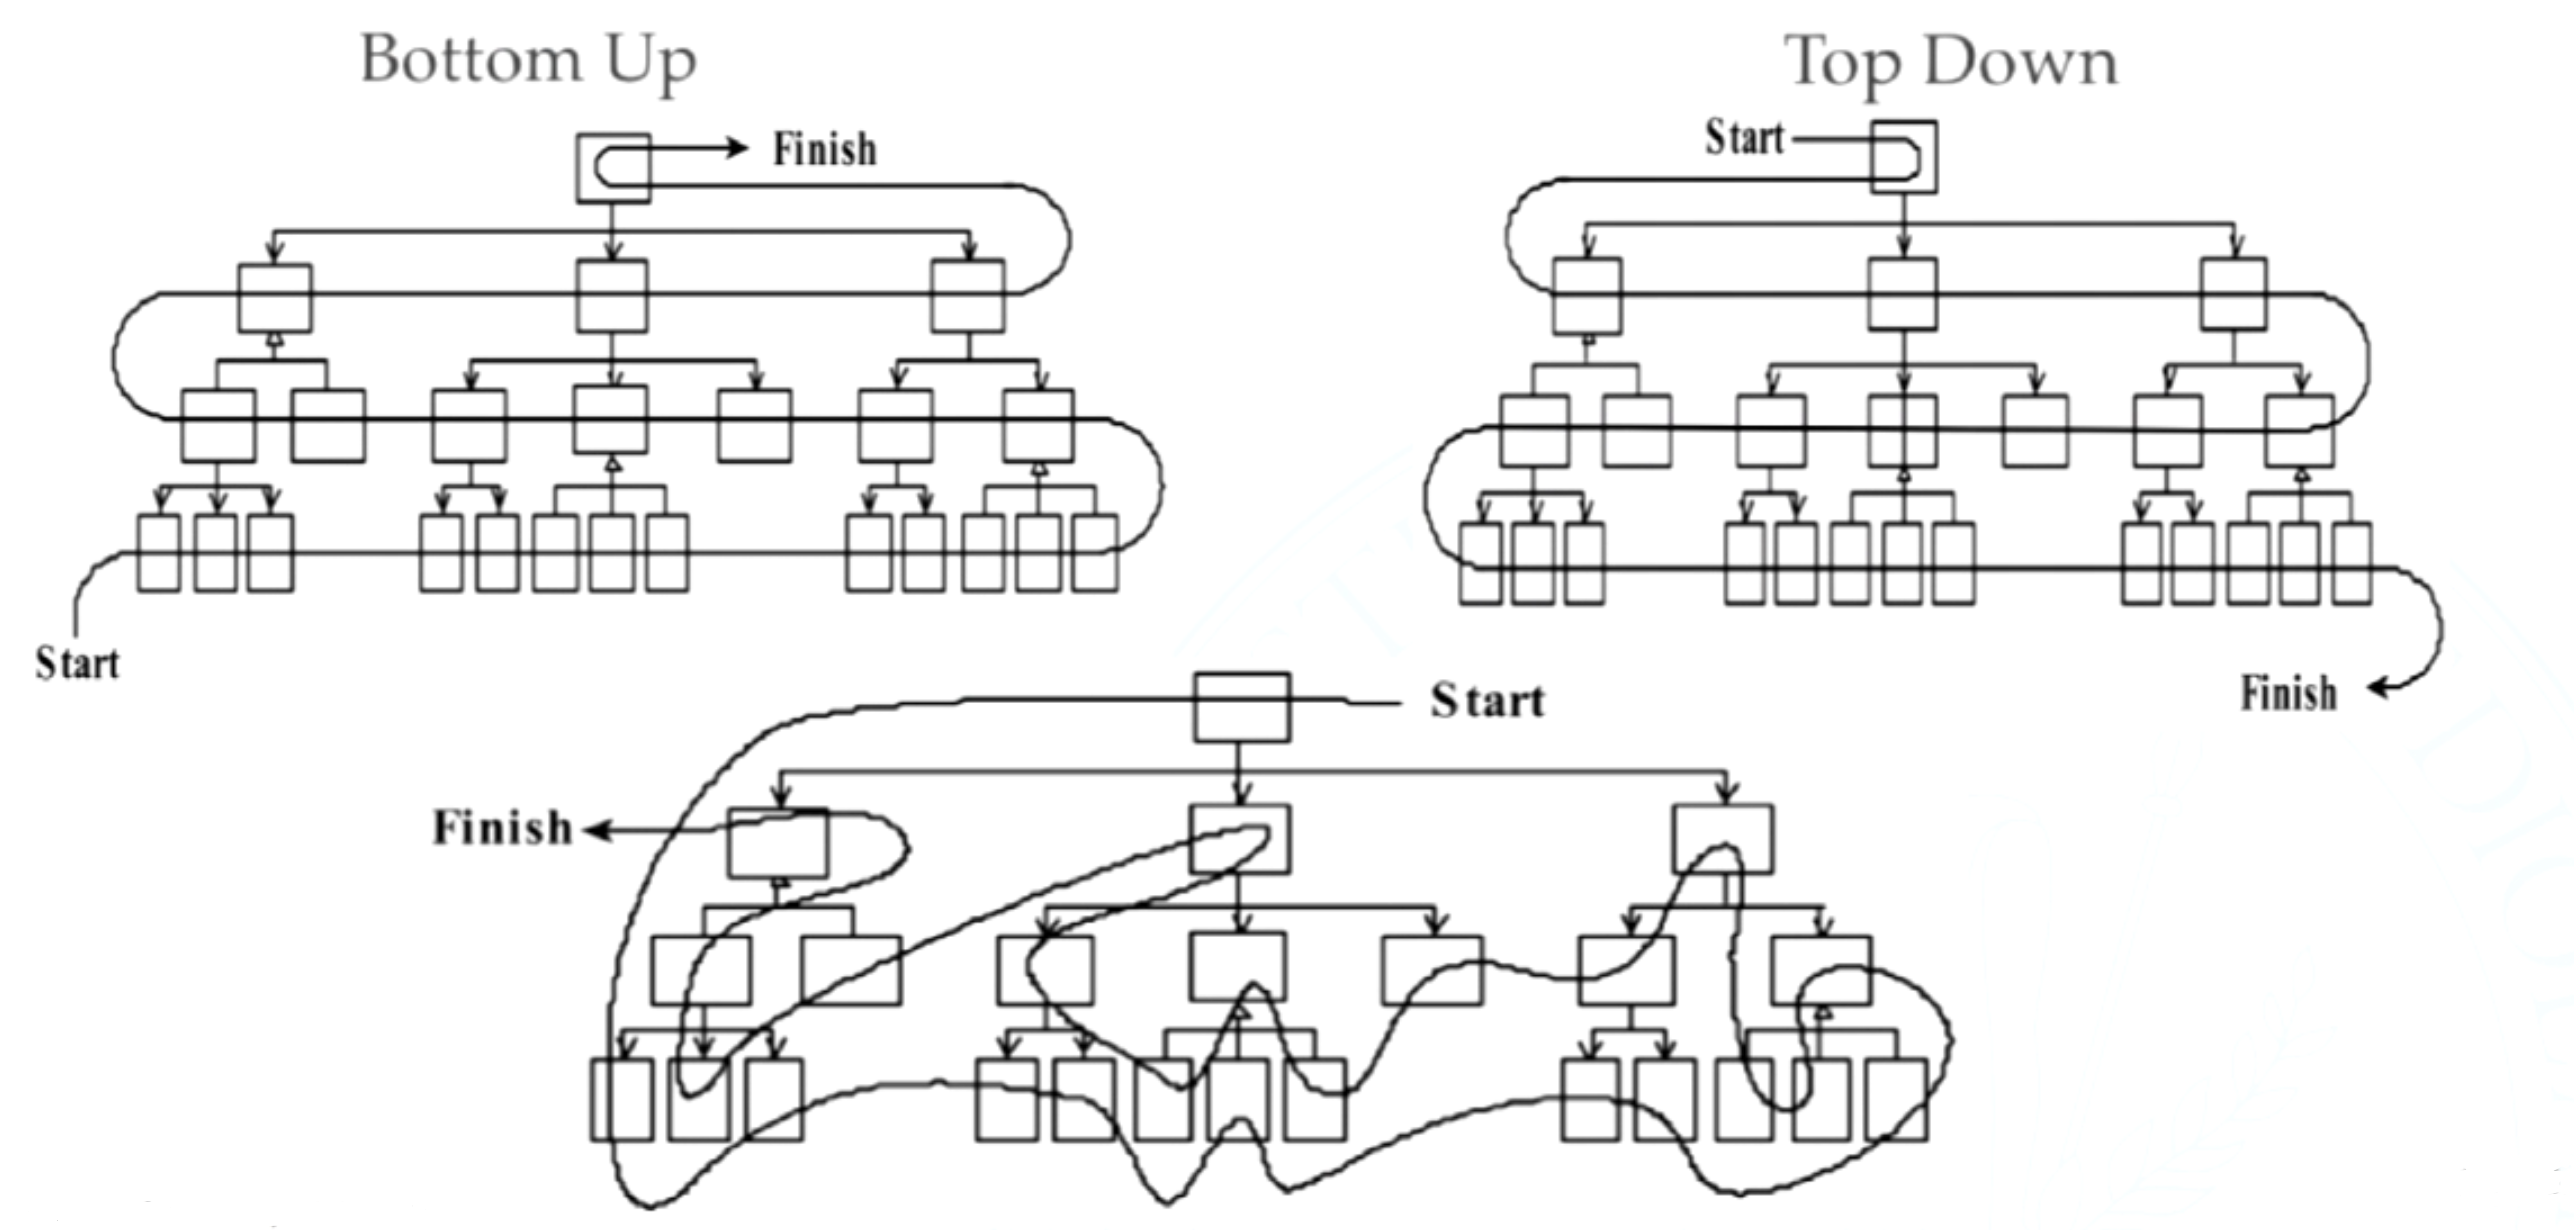
\includegraphics[width=\linewidth]{img/approcci.png}
	 \caption{Diversi tipi di approccio durante gli anni}
\end{figure}
\noindent \textbf{Continuos Integration}: allineamento frequente (molte volte al giorno) dagli ambienti di lavoro degli sviluppatori verso l’ambiente condiviso (mainline).
\\\\
A questo punto l'integrazione non è più fase. Essa viene incorporata nello sviluppo normale. Terminata una parte (una feature, una patch, ...) si integra. Questo però comporta che ogni volta che sviluppo una feature, essa debba essere integrabile. Inoltre, l'integrazione diventa un NONEVENT. Ogni episodio di integrazione ha una durata semplice.

\subsection{Capisaldi (Martin Fowler 2006)}

Martin Fowler nel 2006 formula alcuni principi:
\begin{itemize}
\item \textbf{Mantenere una singola repo}:  tutti devono fare riferimento ad un’unica sorgente in cui ci deve essere tutto, dal codice alla documentazione. Devo avere anche una chiara visione di tutte le vecchie versioni del codice e di quella più recente.
\item \textbf{Automatizzare la build}: l'obiettivo è quello di automatizzare e rendere facilmente ricostruibile il progetto, utilizzando strumenti di automatizzazione di alcune operazioni (quali compilazione, ecc.), tenendo conto anche delle dipendenze. In questo modo risparmio tempo e ho un processo più facile e affidabile. Problematiche:
\begin{itemize}
    \item rischiamo di esagerare nel voler automatizzare a tutti i costi 
    \item automatizzare un task piccolo e poco frequente fa perdere tempo
    \item automatizzare un task può richiedere più tempo del previsto (a causa di debugging, ecc.), il che potrebbe non costituire un vantaggio, ma può renderlo più affidabile.
\end{itemize}
\item \textbf{Build auto-testante}: test automatici eseguiti ogni volta che integro, per controllare che le cose funzionino e che quindi la fase di integrazione abbia avuto successo. Possono essere test di unità e test end-to-end che garantiscono la non regressione, ossia mantenga le funzionalità precedenti.
\item \textbf{Chiunque committa sulla mainline ogni giorno}: ad ogni commit di altre persone, integro i cambiamenti sulla mainline in modo tale da non avere problemi dopo. Siccome posso pushare solo dopo aver risolto i conflitti, l'integrazione avviene sulla mia macchina.
\item \textbf{Ogni commit dovrebbe buildare sulla macchina di integrazione}: le build sono automatizzate. Se falliscono dei test, non consento il push. Il programma non deve funzionare solo sulla propria macchina, ma anche sulla macchina di integrazione.
\item \textbf{Sistemare le build rotte subito}: se i controlli falliscono, quindi l'ultima versione sulla mainline non funziona, va risolto il più velocemente possibile. Si possono adottare tre tipi di soluzione: 
\begin{itemize}
    \item correggere l'errore
    \item tornare ad una versione precedente (revert)
    \item utilizzare una "guardia" che determina l'idoneità rispetto ad una certa serie di test, altrimenti rimane in pending (Git hooks, Gerritt, ecc.).
\end{itemize}
\item \textbf{Mantenere veloce la build}: una build veloce permette di testare ad ogni commit.
\item \textbf{Eseguire i test su un clone dell'ambiente di deployment}: avere una macchina completamente uguale a quella della produzione è indispensabile durante lo staging (per comprendere problemi di retro-compatibilità delle dipendenza, ecc.), in modo da poter verificare che funzioni da entrambe le parti. Docker, permette di isolare i singoli processi e l'ambiente in cui viene eseguito.
\item \textbf{Rendere facile ottenere l'ultimo eseguibile}: fornendo solo il sorgente potrebbe essere che con ambienti di sviluppo diversi il codice non compili. Quindi, bisogna fornire anche gli eseguibili, non solo dell'ultima versione, ma anche delle precedenti.
\item \textbf{Tutti devono poter vedere cosa succede}: bisogna garantire trasparenza, il che vuol dire consentire la visibilità del punto in cui si trova il codice sulla mainline, quali e quanti test ha passato, etc.
\item \textbf{Automate Deployment}: se garantiamo che ci sia sempre nella head della macchina di integrazione la versione più nuova e corretta possiamo automatizzare anche il meccanismo di passaggio in produzione.
\end{itemize}

\begin{figure}[H]
	\centering
	 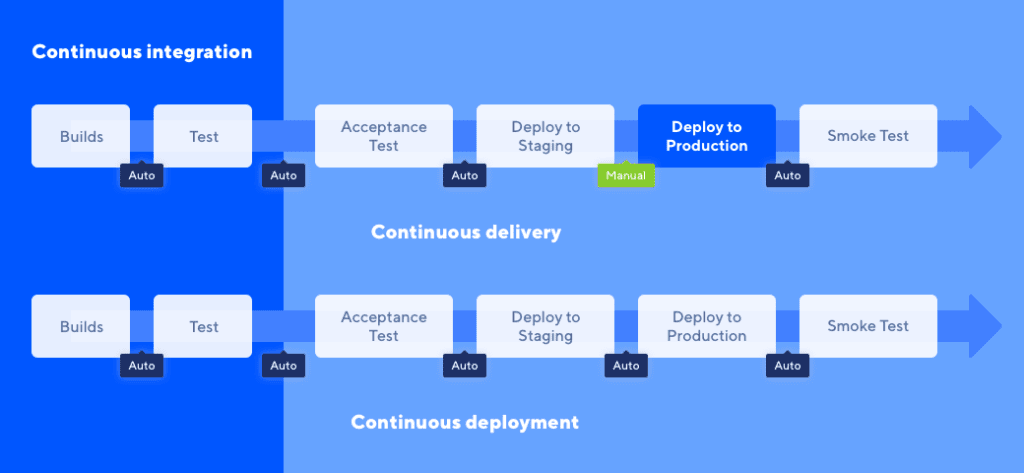
\includegraphics[width=\linewidth]{img/CI-CD.png}
	 \caption{Continuous Delivery vs Continuous Deployment}
\end{figure}

\noindent Non tutto ciò che Fowler riporta in questo articolo è oro colato, essendo un articolo ormai datato. Ad esempio, invita a "tenere i branch al minimo", poiché la gestione dei branch inizialmente era molto complicata. 

\subsection{Configuration Management}
\noindent Dagli anni 70 comincia ad essere utilizzato nel mondo del software.
\\\\
\textbf{Configuration Management}: pratiche che hanno l'obiettivo di rendere sistematico il processo di sviluppo, \textbf{tenendo traccia dei cambiamenti} in modo che il prodotto sia in ogni istante in uno stato (configurazione) ben definito.
\\\\
Gli oggetti di cui si controlla l’evoluzione sono detti configuration item o artifact (manufatto, NON artefatto). Tre scenari di esempio:
\begin{itemize}
    \item Programmatore solo, utile ad esempio per mappare somiglianze tra le versioni
    \item Collaborazione studente professore
    \item Blaming, in modo da sapere per ogni riga di codice chi è stato l'ultimo a modificarla (annotare il listato).
\end{itemize}
L'approccio iniziale era quello di versionare i singoli file, e non l'insieme. Inoltre, per la collaborazione venivano usati sistemi di write lock piuttosto scomodi.
\\
Gli SCM (Source Code Management) sono per lo più indipendenti da linguaggi di programmazione e applicazioni. Lavorano genericamente su file, preferibilmente fatti di righe di testo e calcolando le differenze in base a queste.
\begin{itemize}
    \item anni '80: strumenti locali  (SCCS, rcs, ...)
    \item anni '90: strumenti client-server centralizzati (cvs, subversion, ...)
    \item anni 2000: con l'avvento dell'open source e di internet, si sono resi necessari nuovi metodi di collaborazione \textbf{distribuiti} (peer-to-peer), come git e mercurial. Questo è necessario a permettere una collaborazione da parte di molte persone, anche saltuaria.
\end{itemize}

\subsubsection{Artifact}

\begin{itemize}
    \item Gli artifact sono file o più raramente directory. 
    \item L’SCM permette di tracciare/controllare le revisioni degli artifact e le versioni delle risultanti configurazioni. 
    \item A volte fornisce supporto per la generazione del prodotto a partire da una ben determinata configurazione
\end{itemize}

\subsection{Sincronizzazione}

Il meccanismo di base per controllare l'evoluzione delle revisioni è che ogni cambiamento è regolato da:
\begin{itemize}
    \item check-out dichiara la volontà di cambiare un determinato artifact
    \item check-in (o commit) dichiara la volontà di registrare un determinato change-set
\end{itemize}
Queste vanno a versionare un set di cambiamenti su uno o più file. Non si va quindi a versionare immediatamente ogni linea di codice. Queste operazioni vengono attivate rispetto a un'applicazione di repository. In teoria, non servirebbe un nodo centrale, perchè ogni peer possiede l'intera copia della codebase, che può essere sincronizzata con gli altri. In pratica, si usa un \textbf{repository centrale} per sincronizzare più velocemente e facilmente tutte le modifiche.

\subsubsection{Lavoro concorrente}

L'accesso concorrente si può gestire in due modi:
\begin{itemize}
\item modello pessimistico (rcs): il sistema gestisce l'accesso agli artifact in mutua esclusione attivando un lock al check-out
\item modello ottimistico (cvs): il sistema si disinteressa del problema e fornisce supporto per le attività di merge di change-set paralleli potenzialmente conflittuali.
\end{itemize}

\noindent Il merge rimane un'operazione delicata che generalmente viene trattata con strategie diverse:
\begin{itemize}
\item Lavoro parallelo su artifact diversi
\item Lavoro parallelo sullo stesso artifact, ma su hunk diversi
\item Lavoro parallelo sullo stesso artifact e sullo stesso hunk
\end{itemize}

\noindent Un hunk è un insieme di righe adiacenti che voglio trattare omogeneamente rispetto al mio tool di versioning.
\\\\
\noindent L'ultimo caso necessita sempre di lavoro intelligente. Nel resto dei casi, dipende. Nel caso di lavoro parallelo sullo stesso artifact, quando le due revisioni hanno un antenato comune (per esempio la revisione da cui entrambi sono partiti) si può facilitare il lavoro di merge (3-way merge). Siano A' e A'' due revisioni, con antenato comune A:

\begin{itemize}
    \item hunk uguale nelle tre revisioni: inalterato
    \item hunk uguale in due delle tre revisioni:
    \begin{itemize}
        \item A' e A'' uguali: merge A'
        \item A e A' uguali: merge A''
        \item A e A'' uguali: merge A'
    \end{itemize}
    \item hunk diverso nelle tre revisioni: deve essere valutato a mano
\end{itemize}